% Dit werk is gelicenseerd onder de licentie Creative Commons Naamsvermelding-GelijkDelen 4.0 Internationaal. Ga naar http://creativecommons.org/licenses/by-sa/4.0/ om een kopie van de licentie te kunnen lezen.
\chapter{Stroming in leidingen}
\label{sec:Stroming in leidingen}

%%%%%%%%%%%%%%%%%%%%%%%%%%%%%%%%%%%%%%%%%%%%%%%%%%%%%%%%%%%%%%%%%%%%%%%%%%%%%%%%%%%%%%%%
	\section{Inleiding}
	\label{sec:Stroming in leidingen Inleiding}
In ingenieurstoepassingen komt het vaak voor dat een fluïdum van één plaats naar een andere getransporteerd moet worden. Denk aan de waterleiding die drinkwater van een reservoir tot bij je thuis brengt of de brandstofleiding in een wagen die de brandstof van de tank naar de brandstof injector brengt. De aangewezen manier om dit te doen is door een leiding die volledig met het fluïdum gevuld is. Aangezien het fluïdum in de leiding volledig begrensd is door de leiding spreken we van inwendige stroming. De meest voorkomende leidingen zijn cilindrisch omdat een cirkelvormige sectie geschikt is om hoge drukken te weerstaan. Wanneer het gemiddelde drukniveau in de leiding niet veel groter is dan de atmosfeerdruk kan uit praktische overwegingen ook voor andere doorsnedes gekozen worden. Dit wordt bijvoorbeeld gedaan bij luchtkanalen voor gebouwventilatie die vaak een rechthoekige doorsnede hebben die gemakkelijker in het gebouw te integreren is.

Beschouw nu een vloeistof die een cilindrische leiding instroomt uit een groot reservoir. Wanneer we zeer sterk inzoomen op de grens tussen reservoir en leiding, kunnen we dit benaderen als een vlakke plaat. In het reservoir zal de snelheid quasi uniform zijn. Er zal dus zoals besproken in het hoofdstuk \ref{sec:Uitwendige stroming} een grenslaag ontstaan. Zoals besproken in Sectie \ref{sec:Impulsbalans voor de laminaire stroming over een vlakke plaat} zal de wrijving uitgeoefend door schuifspanningen aan de rand van de leiding gepaard gaan met een daling van de impuls en het verdikken van de grenslaag. Men noemt dit \emph{ontwikkelende stroming}.

Een belangrijk verschil met uitwendige stroming is echter dat de grenslaag zich over de volledige omtrek van de leiding opbouwt. Op een gegeven moment zullen de grenslagen dus samenkomen in het centrum van de leiding (Figuur \ref{fig:Ontwikkelende_stroming}). Verdere opbouw van de grenslaag is dan niet meer mogelijk. Het verder afnemen van de impuls is dus ook niet meer mogelijk. De wrijvingskracht uitgeoefend aan de wanden zal dus door een ander fenomeen opgevangen moeten worden, een drukdaling. Dit type inwendige stroming wordt \emph{volledig ontwikkelde stroming} genoemd.

\begin{figure}[htb]
	\centering
	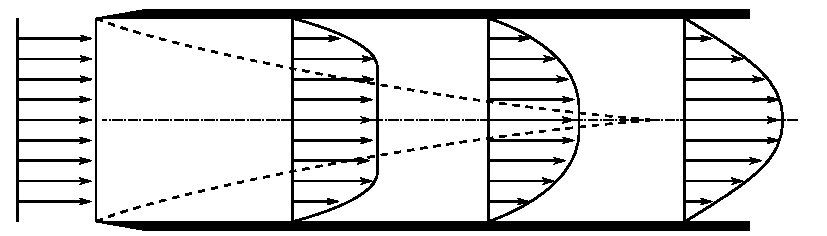
\includegraphics{fig/stroming_in_leidingen/Ontwikkelende_stroming}
	\caption{Opbouw van de grenslaag over de volledige omtrek van een leiding, ontwikkelende stroming}
	\label{fig:Ontwikkelende_stroming}
\end{figure}

%%%%%%%%%%%%%%%%%%%%%%%%%%%%%%%%%%%%%%%%%%%%%%%%%%%%%%%%%%%%%%%%%%%%%%%%%%%%%%%%%%%%%%%%
	\section{Dimensie analyse van de drukval in een cilindrische leiding}
	\label{sec:Dimensie analyse van de drukval in een cilindrische leiding}
Het is interessant om voor het bepalen van de drukval voor specifieke situaties een dimensie analyse uit te voeren. Hiermee kunnen we onze resultaten controleren en in een toepasselijke vorm schrijven.

Uit experimenten, of fysische inzicht kunnen we beredeneren dat de drukval in een cilindrische leiding afhankelijk zal zijn van de lengte van de leiding, de diameter, de gemiddelde snelheid van de stroming, de viscositeit en de dichtheid.
dit kunnen we schrijven als:
\begin{equation}
	\Delta p = \phi(L,D,v,\mu,\rho)
\end{equation}
Volgens het Buckingham-pi theorema kunnen we dus de dimensieloze drukval schrijven als functie van 2 dimensieloze parameters ($n=5$,$k=3$). Deze parameters kunnen we eenvoudig vinden als de relatieve lengte ($L/D$) en het Reynoldsgetal ($\rho v D/\mu = v D/\nu$). Om de druk dimensieloos te maken kunnen we deze delen door de snelheidsdruk ($\frac{1}{2} \rho v^2$):
\begin{equation}
	\frac{\Delta p}{\frac{1}{2}\rho v^2} = f(L/D,Re)
\end{equation}
Uit logische overwegingen moet het drukverlies evenredig zijn met de lengte van de buis:
\begin{equation}
	\frac{\Delta p}{\frac{1}{2}\rho v^2} = \frac{L}{D} f(Re)
	\label{eqn:dimensie analyse drukval laminair}
\end{equation}
Het dimensieloze drukverschil zal dus gelijk zijn aan de relatieve lengte van de buis vermenigvuldigd met een nog onbekende functie van het Reynoldsgetal. Deze onbekende functie noemen we de wrijvingsfactor. We zullen nu trachten het drukverschil te berekenen en in deze vorm te schrijven.
	
%%%%%%%%%%%%%%%%%%%%%%%%%%%%%%%%%%%%%%%%%%%%%%%%%%%%%%%%%%%%%%%%%%%%%%%%%%%%%%%%%%%%%%%%
	\section{Laminaire stroming in een cilindrische leiding}
	\label{sec:Laminaire stroming in een cilindrische leiding}
Beschouw een stationaire, laminaire, volledig ontwikkelde stroming in een cilindrische buis (Figuur \ref{fig:laminaire_stroming_in_buis}).
\begin{figure}[htb]
	\centering
	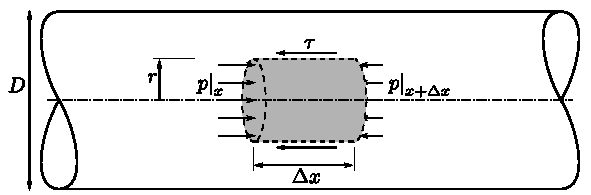
\includegraphics{fig/stroming_in_leidingen/Laminaire_stroming_in_buis}
	\caption{Laminaire stroming in een cilindrische buis}
	\label{fig:laminaire_stroming_in_buis}
\end{figure}
Om het snelheidsprofiel van de stroming uit te rekenen beschouwen we een cilindrisch controlevolume en passen we hier de wet van behoud van impuls (\ref{eqn:controlevolume,behoud van impuls}) op toe in de stroomrichting. Aangezien de stroming stationair is zal de verandering van impuls binnen het controlevolume $0$ zijn. Aangezien de stroming laminair is, is het controlevolume een deel van een stroombuis. De netto uitstroom van impuls uit het controlevolume is dus ook $0$. Vergelijking \ref{eqn:controlevolume,behoud van impuls} wordt dan:
\begin{equation}
	F_x = 0
\end{equation}
De inwerkende krachten bestaan in dit geval uit drukkrachten aan de linker en rechterzijde van het controlevolume en een schuifspanning aan de omtrek van het controlevolume. Dit geeft:
\begin{equation}
	\left. p \pi r^2\right|_{x} - \left. p \pi r^2\right|_{x+\Delta x} -  \tau 2 \pi r \Delta x = 0
\end{equation}
Na deling door $2\pi r \Delta x$ en de limiet te nemen voor $\Delta x$ gaande naar $0$ bekomen we een uitdrukking voor de schuifspanning:
\begin{equation}
	-\frac{1}{2} \frac{\diff p}{\diff x} r= \tau
	\label{eqn:drukgradient}
\end{equation}
Indien we een Newtoniaanse vloeistof veronderstellen kunnen we de schuifspanning schrijven als:
\begin{equation}
	\tau = -\mu \frac{\diff v}{\diff r}
\end{equation}
Het min-teken wordt hier ingevoerd aangezien de afstand tot de wand afneemt met stijgende $r$. Dit resultaat invullen in (\ref{eqn:drukgradient}) geeft:
\begin{equation}
	\frac{1}{2} \frac{\diff p}{\diff x} r = \mu \frac{\diff v}{\diff r}
\end{equation}
Of na omvorming:
\begin{equation}
	\frac{\diff v}{\diff r} = \frac{1}{2 \mu}\frac{\diff p}{\diff x} r
\end{equation}
Deze vergelijking kunnen we integreren over de straal. We bekomen dan een uitdrukking voor de snelheid.
\begin{equation}
	v = \frac{1}{4 \mu}\frac{\diff p}{\diff x} r^2 + C
\end{equation}
De integratie constante $C$ halen we uit de no-slip randvoorwaarde:
\begin{equation}
	\left.v\right|_{r=R} = \frac{1}{4 \mu}\frac{\diff p}{\diff x} R^2 + C  = 0
\end{equation}
Dus:
\begin{equation}
	C = - \frac{1}{4 \mu}\frac{\diff p}{\diff x} R^2
\end{equation}
De het snelheidsprofiel van een stationaire, laminaire, Newtoniaanse vloeistof in een cilindrische buis wordt dan:
\begin{equation}
	v = - \frac{1}{4 \mu}\frac{\diff p}{\diff x} R^2 \left(1- \frac{r^2}{R^2}\right)
\end{equation}
We vinden een kwadratisch snelheidsprofiel terug met als maximale snelheid:
\begin{equation}
	v_{\text{max}} = - \frac{1}{4 \mu}\frac{\diff p}{\diff x} R^2
\end{equation}
We kunnen het snelheidsprofiel dus dimensieloos schrijven als:
\begin{equation}
	\frac{v}{v_{\text{max}}} = \left(1- \frac{r^2}{R^2}\right)
\end{equation}
Een stroming met dit soort snelheidsprofiel wordt Poiseuille stroming genoemd naar de Franse fysicus Jean Louis Marie Poiseuille en is weergegeven in Figuur \ref{fig:laminair_snelheidsprofiel}:
\begin{figure}[htb]
	\centering
	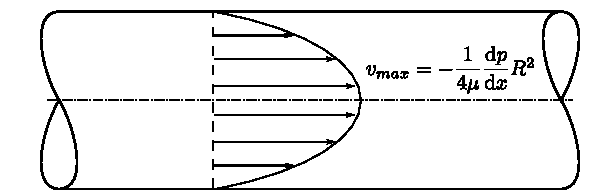
\includegraphics{fig/stroming_in_leidingen/Laminair_snelheidsprofiel}
	\caption{Snelheidsprofiel bij laminaire stroming in een cilindrische buis}
	\label{fig:laminair_snelheidsprofiel}
\end{figure}

Voor het maken van berekeningen is het interessant om de drukverandering te kunnen schrijven in functie van de gemiddelde snelheid in de buis. We kunnen de gemiddelde snelheid in de buis berekenen door het debiet te delen door de oppervlakte. Het debiet in de buis kan berekend worden als de integraal van de snelheid over de volledige oppervlakte:
\begin{equation}
	\dot{V} = 2 \pi \int_0^R v_{\text{max}} \left(1- \frac{r^2}{R^2}\right) r \diff r = v_{\text{max}} \frac{\pi R^2}{2}
\end{equation}
De gemiddelde snelheid wordt dan:
\begin{equation}
	v_{\text{gem}} = \frac{v_{\text{max}}}{2} = - \frac{1}{8 \mu}\frac{\diff p}{\diff x} R^2
\end{equation}
Voor ingenieurs is het handiger om met de diameter $D$ van de buis te werken in plaats van met de straal $R$. We kunnen het drukverlies over een horizontale leiding met lengte $L$ dan uitdrukken als:
\begin{equation}
	\Delta p = - 32 \mu \frac{v_{\text{gem}} L}{ D^2}
\end{equation}
Uit de dimensie analyse weten we dat de drukval afhankelijk moet zijn van $\frac{1}{2}\rho v^2$ aangezien deze samen de dimensieloze drukcoëfficiënt vormen. Indien we het vorige resultaat herschrijven bekomen we inderdaad:
\begin{equation}
	\Delta p = 64 \frac{1}{2}\rho v^2 \frac{\mu}{\rho v D} \frac{L}{D} = \frac{64}{Re} \frac{1}{2}\rho v^2 \frac{L}{D}
	\label{eqn:drukval bij laminaire stroming}
\end{equation}
We hebben nu een vergelijking om de drukval over een cilindrische leiding voor laminaire, niet-samendrukbare stroming te berekenen. Deze vergelijking staat bekend als de wet van Hagen-Poiseuille. Hierin is de drukcoëfficiënt afhankelijk van twee dimensieloze combinaties, $64/Re$ en $L/D$, zoals voorspeld in sectie \ref{sec:Dimensie analyse van de drukval in een cilindrische leiding}. Voor laminaire stroming is de wrijvingsfactor $f$ dus gelijk aan $64/Re$.

%%%%%%%%%%%%%%%%%%%%%%%%%%%%%%%%%%%%%%%%%%%%%%%%%%%%%%%%%%%%%%%%%%%%%%%%%%%%%%%%%%%%%%%%
	\section{Turbulente stroming}
	\label{sec:Turbulente stroming}

Wanneer de diameter van de buis of de snelheid in de buis groot genoeg is zal de stroming in de buis niet meer laminair zijn. Er zijn fluctuaties in de snelheid die ervoor zorgen dat het snelheidsprofiel niet meer stationair is. Dit gedrag werd experimenteel waargenomen door Osbourne Reynolds. Hij zag dat wanneer de dimensieloze combinatie $\frac{v D}{\nu}$ laag genoeg bleef, de stroming in een buis laminair was. De dimensieloze combinatie is dan ook naar hem vernoemd en kennen we als het Reynoldsgetal.

In cilindrische buizen blijft de stroming laminair tot een Reynoldsgetal van ongeveer 2300. Bij een Reynoldsgetal groter dan 10000 zal de stroming daarentegen meestal turbulent zijn. Bij Reynoldsgetallen tussen 2300 en 10000 is het zowel mogelijk dat de stroming laminair of turbulent is. Deze zone noemt met het overgangsgebied.

Wanneer we dit vergelijken met de waarnemingen die we gedaan hebben bij de vlakke wand in Sectie \ref{sec:Grenslagen}, zien we een gelijkaardig gedrag. In een buis zal er een axis-symmetrische grenslaag ontstaan die in het midden van de buis samenkomt. Wanneer de diameter van de buis dus klein genoeg blijft (kleiner dan de kritische grenslaag dikte) zal de stroming laminair blijven. Wanneer de diameter van de buis groter wordt, wordt de stroming turbulent. Ook de manier waarop de weerstandskracht uitgeoefend wordt verloopt gelijkaardig. In het centrale turbulente gedeelte is er impulsoverdracht (of wrijving) door de onregelmatigheid van de snelheid (turbulente schuifspanning). In de laminaire sublaag dicht bij de wand is er wrijving door de viscositeit (laminaire schuifspanning). Er ontstaat dus een centraal vlakker gemiddeld snelheidsprofiel met een zeer plots overgang aan de wanden van de buis (Figuur \ref{fig:turbulent_snelheidsprofiel}). Deze grote snelheidsgradiënt brengt grote schuifspanningen en dus een grotere drukval met zich mee.

In de literatuur zijn verschillende experimentele correlaties voor het gemiddelde snelheidsprofiel van een turbulente stroming terug te vinden. Een correlatie met aanvaardbare nauwkeurigheid en eenvoudig gebruik is het \emph{power-law} snelheidsprofiel \cite{Munson2010}:
\begin{equation}
	\frac{\bar{v}}{v_{\text{max}}} = \left(1- \frac{r}{R}\right)^{1/n}
\end{equation}
Waarbij $n$ een functie is van het Reynoldsgetal van de stroming. Een waarde van $n=7$ wordt vaak gebruikt aangezien dit steeds een redelijke benadering geeft. Hoewel de waarde van de snelheid goed benaderd wordt, wordt de snelheidsgradiënt in de buurt van de wand en op de aslijn niet goed weergegeven. Aan de wand gaat de gradiënt naar oneindig terwijl deze op de aslijn niet $0$ wordt.
\begin{figure}[htb]
	\centering
	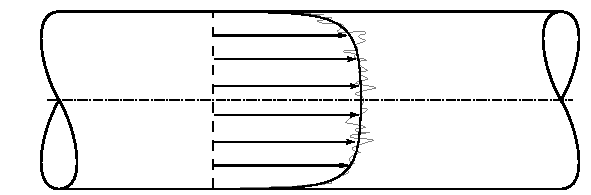
\includegraphics{fig/stroming_in_leidingen/Turbulent_snelheidsprofiel}
	\caption{Snelheidsprofiel bij turbulente stroming in een cilyndrische buis}
	\label{fig:turbulent_snelheidsprofiel}
\end{figure}

Bij metingen van het drukverlies bij turbulente stroming door een horizontale buis blijkt dat deze afhankelijk wordt van het type buis dat gebruikt werd. Meer bepaald de ruwheid van de buis zal een rol te spelen. We zullen dus (\ref{eqn:dimensie analyse drukval laminair}) moeten aanpassen. Dit kan eenvoudig door de relatieve ruwheid te definiëren als de ruwheid gedeeld door de diameter. De dimensieloze relatie wordt dan:
\begin{equation}
	\frac{\Delta p}{\frac{1}{2}\rho v^2} = \frac{L}{D} f(Re,\varepsilon/D)
	\label{eqn:dimensie analyse drukval turbulent}
\end{equation}
De wrijvingsfactor wordt dus afhankelijk van het Reynoldsgetal en de relatieve ruwheid (De gebruikte waarde van ruwheid komt overeen met de diameter van de ruwheidskorrels). De verschillende afhankelijkheid van de drukval van de relatieve ruwheid bij laminaire en turbulente stroming kunnen we verklaren door naar de laminaire sublaag aan de wand van de buis te kijken (Figuur \ref{fig:Invloed_ruwheid}). Wanneer de wand ruw is zullen de ruwheidspieken tot ver in de laminaire sublaag doordringen. Aangezien bij turbulente stroming grootste deel van de wrijving in deze laminaire sublaag wordt gegenereerd zal de ruwheid een invloed hebben op de weerstand. Bij laminaire stroming strekt de laminaire laag zich uit over heel de buis. De ruwheid dringt dus slechts in een zeer klein deel hiervan door en zal dus bijna geen invloed hebben op de totale weerstand.
\begin{figure}[htb]
	\centering
	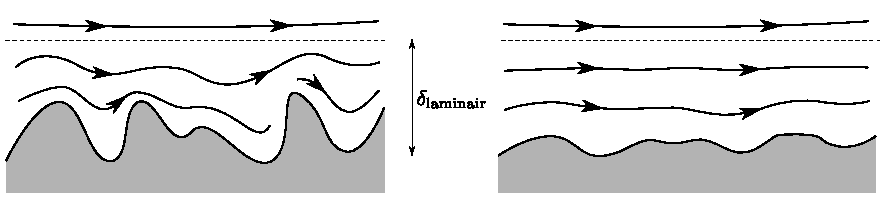
\includegraphics{fig/stroming_in_leidingen/Invloed_ruwheid}
	\caption{De invloed van de relatieve ruwheid op de laminaire sublaag}
	\label{fig:Invloed_ruwheid}
\end{figure}

Waarden van karakteristieke ruwheden voor verschillende materialen zijn weergegeven in Tabel \ref{tab:ruwheid van materialen}
\begin{table}[htb]
	\centering
	\begin{tabular}{cc}
		\hline
		Oppervlak & Ruwheid \\
		   & (mm) \\
		\hline
		Commercieel glad messing, lood, koper of kunststof & 0.0015 \\
		Staal en smeedijzer & 0.046 \\
		Gegalvanizeerd staal of ijzer & 0.152 \\
		Gietijzer & 0.259 \\
		\hline
	\end{tabular}
	\caption{Karakteristieke ruwheidswazarden voor verschillende materialen (uit ASHRAE Handbook of Fundamentals \cite{ASHRAE_Fundamentals})}
	\label{tab:ruwheid van materialen}
\end{table}
Het drukverlies wordt dus:
\begin{equation}
	\Delta p = f \frac{1}{2}\rho v^2 \frac{L}{D}
	\label{eqn:drukval bij turbulente stroming}
\end{equation}

Na vele experimenten door onder andere Johann Nikuradse \cite{Nikuradse1926} werd de relatie tussen de wrijvingsfactor, het Reynoldsgetal en de relatieve ruwheid vastgesteld. Deze relatie kan benaderd worden door de formule van Colebrook \cite{Colebrook1937}. Deze heeft een relatieve nauwkeurigheid van 5\% voor gladde leidingen en 10\% voor ruwe leidingen.
\begin{equation}
	\frac{1}{\sqrt{f}} = -2 \log \left( \frac{\varepsilon/D}{3.72} + \frac{2.51}{Re \sqrt{f}} \right)
\end{equation}
Dit is een impliciete formule die niet in gesloten vorm naar $f$ kan worden opgelost. Ze kan wel iteratief worden opgelost.  Om dit probleem te verhelpen wordt de wrijvingsfactor in grafische vorm weergegeven in het Moody diagram (Appendix \ref{fig:Moody diagram}) genoemd naar Lewis F. Moody die het als eerste voorstelde in 1944 \cite{Moody1944}.

Wanneer we het diagram bestuderen zien we dat bij grote waarden van het Reynoldsgetal de wrijvingsfactor niet meer afhankelijk is van het Reynoldsgetal maar enkel nog van de relatieve ruwheid. In dit geval wordt de stroming volledig ruw genoemd.

		\subsection{Stroming door niet cilindrische buizen}
Bij volledig ontwikkelde stroming door volledig gevulde niet cilindrische buizen of kanalen kunnen gelijkaardige formules als hierboven toegepast worden op voorwaarde dat de diameter $D$ van de buis wordt vervangen door de hydraulische diameter $D_h$ gedefinieerd als:
\begin{equation}
	D_h = \frac{4 A}{P}
\end{equation}
Met $A$ de doorstroom sectie en $P$ de bevochtigde omtrek van de sectie.
	


